\chapter{Preliminaries \label{chap:Preliminaries}}


We will start with a  description of transport processes in QDs which will lead us to talk about the Anderson model. Then we will take a look to the Kondo effect and, in particular, to its consequences in quantum dots.  

%-------------------------------------------------------------
%Here goes the introduction of transport between quantum dots. stil need to add important considerations like the smooth varying DOS. Not so discrete. 
%Assumption: 
%   1-Only the level immediately at the bottom of the fermi       level is considered
\section{Transport in Quantum Dots (QDs)}
% --------------Figure-------------------------
\begin{figure}[hbt]
    \centering
    \subfloat[\label{QD-figuresA}\label{QD-figures}]{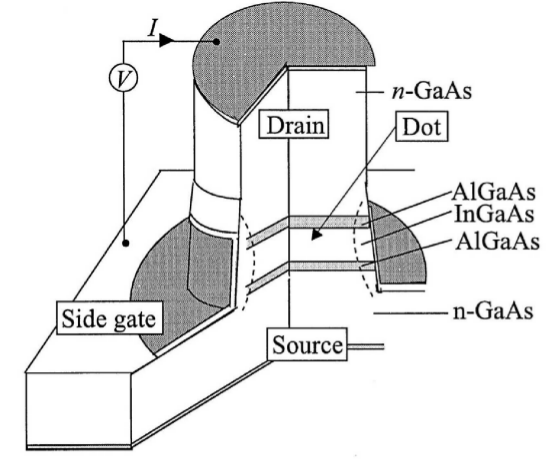
\includegraphics[scale=0.3]{IMAGES/Preliminars/VerticalQD.png}}\hspace{6mm}
    \subfloat[\label{QD-figuresB}]{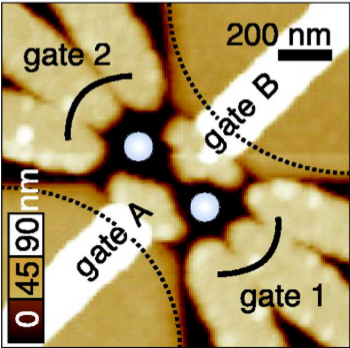
\includegraphics[scale=0.4]{IMAGES/Preliminars/QD-horizontal.png}}
    \caption{ a) Vertical quantum dot.  b)Atomic force microscopy
    picture of two coupled lateral QDs (bright central circles). Gates 1 and 2 act as drain and source voltage. A negative
    voltage is applied at gates $A$,$B$ to allow the formation of the droplets inside the free space in the 2D electron gas. \protect\Source{\cite{holleitner_probing_2002}} }
\end{figure}

Quantum mechanical effects are visible when the system size is of the order of the de Broglie wavelength \citep[(1.1)]{bimberg_quantum_1999}
\[
\lambda_{f}=\frac{h}{\sqrt{3m_{\mathsf{eff}}k_{B}T}}
\]
 where $m_{\mathsf{eff}}$ is the electron effective mass in the crystal.
Since $m_{\mathsf{eff}}$ can be much smaller than the free electron mass in some semiconducting materials, size quantization effects can be observed at system of sizes $\sim100\mbox{nm}$ \citep[2.1]{sindel_numerical_2005}. A device confined in the three dimensions up to this length-scale will present the behavior of a $0$D quantum system, which is what we call a Quantum Dot (QD).\\

\begin{figure}[tb]
    \centering
    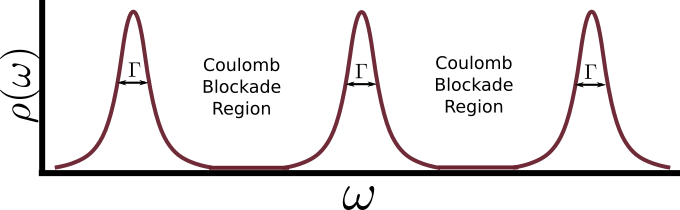
\includegraphics[scale=0.5]{IMAGES/Preliminars/specDot.png}
    \caption{Pictorial representation of the Density of States of a QD. The gate potential $V_G$ can be tuned to change the fermi energy of the dot.  \protect\Source{By the author} }
    \label{fig:specDots}
\end{figure}


\begin{figure}[t]
     \centering
    
     \subfloat[ \label{fig:QD-transport}]{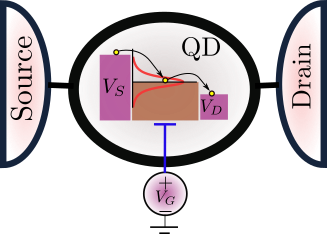
\includegraphics[scale=0.7]{IMAGES/Preliminars/QD-Transport.png}}
    \subfloat[\label{fig:QD-Blockade}]{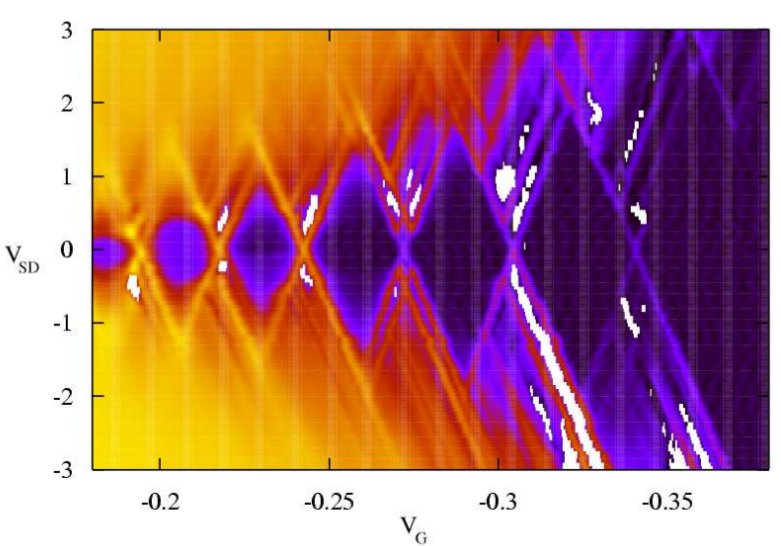
\includegraphics[scale=0.3]{IMAGES/Preliminars/QD-Blockade.png}}
     \caption{ a) Representation of transport through QD. The red curve represents the hybridized energy level. The gate voltage tunes this level. In the case represented, the energy level is in the middle of the drain and source voltages allowing transport between the leads.   Charging diagram of a quantum dot. b) Plot of the conductance vs the gate voltage $V_G$ and the source-drain voltage $(V_{SD}=V_{S}-V_{D} )$ \protect\Source{a) By the Author , b) \cite{sindel_numerical_2005}  }}
\end{figure}

Nowadays, QDs can be manufactured with several methods, forms and orientations \citep{bimberg_quantum_1999}. According to their orientation with respect to the based 2D-plane , two main types of QDs can be distinguished : Vertical (Figure \ref{QD-figuresA}) and lateral (Figure \ref{QD-figuresB}) QDs. Both types of of quantum dots have $3$-main gates. Two of them are the Drain $V_D$ and source $V_S$ gate voltages used to control the current trough the QD. The third one is the gate voltage $V_G$. This one controls the electron confinement inside the QD. Therefore, tuning the gate voltage it is possible to control accurately the energy levels of the QD. 

% \begin{figure}[t]
%     \centering
%     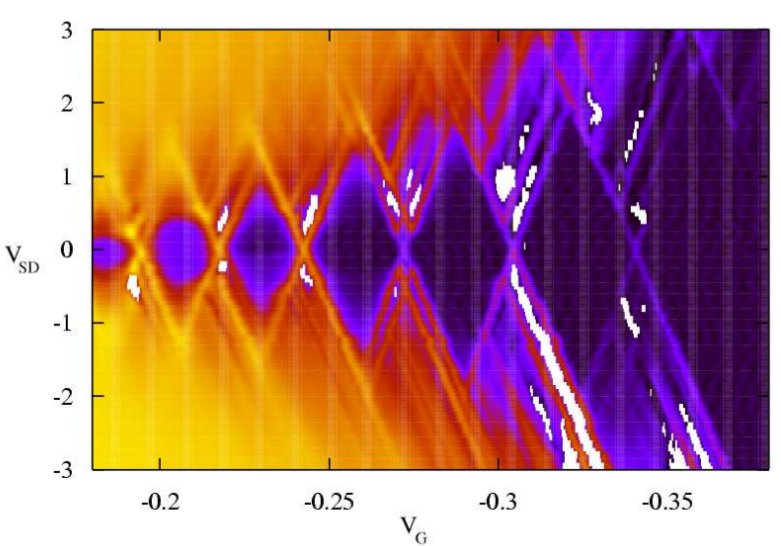
\includegraphics[scale=0.3]{IMAGES/Preliminars/QD-Blockade.png}
%     \caption{ Charging diagram of a quantum dot. The conductance is plotted vs the gate voltage $V_G$ and the source-drain voltage $(V_{SD}=V_{S}-V_{D} )$ \protect\Source{\cite{sindel_numerical_2005} } }
%     \label{fig:QD-Blockade}
% \end{figure}


Ideally, the energy spectrum of a QD is a discrete set of energy levels resembling the spectrum of an atom. However, when the QD is connected to metallic leads these energy levels hybridized with respect to a hybridization parameter $\Gamma$ which depends on the voltage connecting the lead with the dots $V$ as 
\begin{equation}
    \Gamma \propto \pi \Vert V \Vert^2
\end{equation}

in a flat band. A representation of this fact can be found in  \ref{fig:specDots}. Ideally, $\Gamma \ll \Delta E$ such that the energy levels do not overlap each other. In addition the gate voltage allows us to tune the energy levels of the QD.

To execute transport measurements the QD must be attached to two leads (See \ref{fig:QD-transport}). Each lead will have a characteristic gate voltage $V_S$ (Left lead) and $V_D$ (Right lead). An electron can pass from the source to the drain if there is an energy level in the middle of the two voltages, just as in \ref{fig:QD-transport}. However if this condition is not satisfied the dot enters into a coulomb blockade region without  electron transport between both leads as can be observed in \ref{fig:QD-Blockade}. Inside the coulomb blockade regions the number of electrons is constant. When increasing $V_G$ a single electron enters into the dot each time. Since all of these effects can be controlled by a tuning the gate voltage, the system described is indeed a single electron transistor (SET).  






% Indeed we can model an ideal single-electron QD as a quantum well
% with a negative constant potential inside the dot . For example an
% spherical quantum dot with radius $R$ will take the following Schr�dinger
% Hamiltonian 

% \[
% H\Psi(r)=\left(\frac{\hbar^{2}}{2m^{*}}\nabla^{2}+V(r)\right)\Psi(r)\ ,\ \textrm{with }V(r)=\begin{cases}
% -V_{0} & r<R\\
% 0 & r\geq R
% \end{cases}.
% \]


% The 
% the energy level spacing is  \citep[Equation (5.44)]{bimberg_quantum_1999}

% \[
% \delta E\propto\frac{1}{R^{2}}.
% \]



%------------------------------------------------------------
\section{The Anderson Model}
The Anderson model \citep{anderson_localized_1961} was originally designed to study the physics of magnetic impurities, which makes it a perfect model to study the Kondo Effect that we will describe in the following section. However,  QDs also behave like magnetic impurities. Hence the physics of QDs can be studied using the Anderson model.

Moreover, there are two regimes that  will be particularly important in this thesis.  They depend on whether Coulomb repulsion is important or not. These are
\begin{itemize}
    \item \textbf{Non-interacting systems:} This means the coulomb repulsion is not relevant . In this case, spin-$\uparrow$ and spin-$\dw$ channels are independent which simplifies many of the procedures. The method used to describe solve this systems is ballistic transport. 
    \item \textbf{Interacting systems:} The coulomb repulsion is relevant. The repulsion factor will be defined by the factor $U$. In this case, the spin-$\uparrow$ and spin-$\dw$ channels are not independent since the coulomb repulsion limits the number of particles inside each dot. We will use the Numerical Renormalization Group to treat this kind of systems.  
\end{itemize}


The Anderson model takes in account both regimes and  the only difference in each case will be the value of $U$ parameter ($U=0$ non-interacting , $U>0$ interacting). Taking this in account we proceed to present the Anderson model in QDs.

Using the Hunds rules we know that the energy levels inside the dot should be filled from lower to higher energies with two electrons with different spin at each state. Each pair of electrons will interact magnetically and electrically. In addition, there is and energy associated to each electron and a Zeeman splitting factor in case a $\hat{z}$-directed magnetic field $B$ is placed.  Considering these interactions we can obtain a very general expression in second quantization for the QD Hamiltonian
of the form \citep[(3.2)]{sindel_numerical_2005}

\[
H_{d}=\sum_{i\sigma}\epsilon_{di}d_{i\sigma}^{\dagger}d_{i\sigma}+\sum_{i}U_{i}\hat{n}_{i\uparrow}\hat{n}_{i\downarrow}+\sum_{\sigma\sigma',i\neq j}U_{ij}\hat{n}_{i\sigma}\hat{n}_{j\sigma'}-\mu_{B}gB\sum_{i}S_{i}^{z}+J\sum_{i\neq j}\mathbf{S}_{i}\cdot\mathbf{S}_{j}.
\]


Where $\sigma\in\{\uparrow,\downarrow\}$, $d_{i\sigma}^{\dagger}\left(d_{i\sigma}\right)$
is the dot creation(annihilation) operator,$\hat{n}_{i\sigma}:=d_{i\sigma}^{\dagger}d_{i\sigma}$
is the particle number, $\mathbf{S}_{i}$ is the spin-vector, $\epsilon_{di}$
is the energy of the $i^{\mbox{th}}$-level in the dot, $U_{i}$ is
the coulomb repulsion between electrons in the same energy level $i$,
$U_{ij}$ is the coulomb interaction between electrons in different
levels (And therefore smaller than $U_{i}$), \textbf{$B$} is an
applied magnetic field in the $\hat{z}$-direction and $J$ is the
term representing the Zeeman splitting. 

At low temperatures, the main interactions only with the level closest to the Fermi energy. This allows us to make the single-level approximation, neglecting the other energy levels. This assumption reduces the complexity of the dot Hamiltonian to \\


\begin{equation}
    H_{d}=\sum_{\sigma}\epsilon_{d}d_{\sigma}^{\dagger}d_{\sigma}+U\hat{n}_{\uparrow}\hat{n}_{\downarrow}-\mu_{B}gBS^{z}. \label{eq:hdot}
\end{equation}





The lead hambiltonian is decomposed in two hamiltonians. The energy of the electrons inside the leads $H_{lead}$ and the interaction between the leads and the quantum dot $H_{int}$. These hamiltonians take the form 

\begin{eqnarray*}
H_{lead} & = & \sum_{\mathbf{k}\sigma l}\epsilon_{\mathbf{k}l}c_{\mathbf{k}\sigma l}^{\dagger}c_{\mathbf{k}\sigma l}\\
H_{int} & = & \sum_{\mathbf{k}\sigma l}V_{\mathbf{k}l}c_{\mathbf{k}\sigma l}^{\dagger}d_{\sigma}+V_{\mathbf{k}l}^{*}d_{\sigma}^{\dagger}c_{\mathbf{k}\sigma l},
\end{eqnarray*}


where $\mathbf{k}$ represents the possible crystal momentums in the
leads, $l\in\{S,D\}$, $c_{\mathbf{k}\sigma l}^{\dagger}(c_{\mathbf{k}\sigma l})$
creates(annihilates) an electron with momentum $\mathbf{k}$ and spin
$\sigma$ in the lead $l$, $\epsilon_{\mathbf{k}l}$ is the energy
of the electron in the leads and $V_{\mathbf{k}l}$ is a hopping exchange
term between the leads and the QD. 


In conclusion the sum of these three interactions is receives the name of Anderson Model. 
\begin{eqnarray}
H & = & H_{d}+H_{lead}+H_{int}\nonumber \\
 & = & \sum_{\sigma}\epsilon_{d}d_{\sigma}^{\dagger}d_{\sigma}+U\hat{n}_{\uparrow}\hat{n}_{\downarrow}-\mu_{B}gBS^{z}+\sum_{\mathbf{k}\sigma l}\epsilon_{\mathbf{k}l}c_{\mathbf{k}\sigma l}^{\dagger}c_{\mathbf{k}\sigma l}+\sum_{\mathbf{k}\sigma l}V_{\mathbf{k}l}c_{k\sigma l}^{\dagger}d_{\sigma}+V_{\mathbf{k}l}^{*}d_{\sigma}^{\dagger}c_{\mathbf{k}\sigma l}.\label{eq:Anderson}
\end{eqnarray}

For this project, we will make two extra changes to the Anderson model. Using the anti-commutation properties of the fermion operators

% \begin{equation}
% H=H_{d}+H_{lead}+H_{int}=\sum_{\sigma}\epsilon_{d}d_{\sigma}^{\dagger}d_{\sigma}+U\hat{n}_{\uparrow}\hat{n}_{\downarrow}+\sum_{\mathbf{k}\sigma l}\epsilon_{\mathbf{k}l}c_{\mathbf{k}\sigma l}^{\dagger}c_{\mathbf{k}\sigma l}+V_{\mathbf{k}l}c_{\mathbf{k}\sigma l}^{\dagger}d_{\sigma}+V_{\mathbf{k}l}^{*}d_{\sigma}^{\dagger}c_{\mathbf{k}\sigma l}.\label{eq:hamB0}
% \end{equation}
\[
\left\{ d_{\sigma}^{\dagger},d_{\sigma'}\right\} =\delta_{\sigma\sigma'}\ ,\ \left\{ d_{\sigma}^{\dagger},d_{\sigma'}^{\dagger}\right\} =\left\{ d_{\sigma},d_{\sigma'}\right\} =0
\]
we get


\begin{eqnarray*}
\left(d_{\up}^{\dagger}d_{\up}+d_{\down}^{\dagger}d_{\down}-1\right){}^{2} & = & \sum_{\sigma}\left(d_{\sigma}^{\dagger}d_{\sigma}\right)^{2}-2\sum_{\sigma}d_{\sigma}^{\dagger}d_{\sigma}+2d_{\up}^{\dagger}d_{\up}d_{\down}^{\dagger}d_{\down}-1\\
 & = & 2d_{\up}^{\dagger}d_{\up}d_{\down}^{\dagger}d_{\down}-\sum_{\sigma}d_{\sigma}^{\dagger}d_{\sigma}-1.
\end{eqnarray*}

Replacing this in \eqref{eq:hdot} we obtain a  nice spin-symmetric form of the dot hamiltonian

\begin{equation}
    \left(\epsilon_{d}+\frac{U}{2}\right)d_{\sigma}^{\dagger}d_{\sigma}+\frac{U}{2}(d_{\sigma}^{\dagger}d_{\sigma}-1)^{2}-\mu_{B}gBS^{z}. 
    \label{eq:hdot2}
\end{equation}

In addition, it is possible to do a linear transform to the lead opperators 
\begin{equation}
    \frac{1}{\sqrt{V_{S}^{2}+V_{R}^{2}}}\left[\begin{array}{cc}
V_{S} & V_{R}\\
-V_{R} & V_{S}
\end{array}\right]\left[\begin{array}{c}
c_{\mathbf{k}\sigma S}\\
c_{\mathbf{k}\sigma D}
\end{array}\right]=\left[\begin{array}{c}
c_{\mathbf{k}\sigma+}\\
c_{\mathbf{k}\sigma-}
\end{array}\right]
\end{equation}
After the transformation the operator will be decoupled from the dot hamiltonian $c_{\mathbf{k}\sigma-}$ . This implies that we can suppose that the  \textbf{dot is coupled wit just one lead}. During the rest of the thesis we will mantain this convention. 


%------------------------------------------------------------
\section{Kondo Effect}

\Jesus{Here goes a review about the Kondo Effect. I am still trying to figure out how it section will look like. For now Im just leaving some ideas and plots.}\\

In the early 30s the physicist where intrigued by the observation of a resistance minimum in some metals at low temperatures $(\sim 10K)$ \cite{sindel_numerical_2005} . The phenomenon received the name of Kondo effect \citep{hewson_kondo_1997}. This effect is attributed to the electron-scattering with the magnetic impurities present in the materials. 

Using perturbation theory is possible to explain how this spin flip produces a  temperature dependent effect which  introduces an additional logarithmic term to the resistivity of the form

\begin{equation}
\rho_{Kondo}(T) \propto \ln{\left( \frac{T_{kondo}}{T} \right)},
\label{logKondo}
\end{equation}



which occurs due to the spin-flip between the particles in the impurity and in the reservoir. The entire resistivity including  and 

We can seen that under the scale of temperature defined by $T_k$ the Kondo effect dominates over all other interactions. However, there is a fundamental problem in the Kondo model. For temperatures much smaller than $T_K$ the resistivity diverges. This problem is solved by applying a re-normalization group approach to treat the strong correlations appearing at low temperatures. In the Kondo problem a logarithmic discretization is used. The numerical procedure receives the name of Numerical renormalization Group (NRG). 


\subsection{Kondo Effect in QDs}


The problem of magnetic impurities in metals can be treated using the Anderson model in a similar form as the transport
 in quantum dots. Hence, it is not a surprise that Kondo Effect could also occur in QDs. When an odd number of electrons is in the QD the last level bellow the Fermi energy is half-occupied and hence the dot is magnetized. The unlocalized electrons in the reservoirs then interact with this localized electron . Spin-flip can occur as in the case of  magnetic impurities in metals. At low temperatures, this magnetic  interaction gives rise to strong quantum correlations that favor the formation of a singlet state between the localized electron and the electrons in the leads. As a result, the zero-bias density of states is increased producing a zero-bias conductance peak. \\

Note that the physical implications of the Kondo effect  between the case of magnetic impurities in metals and transport through QD are different. The reason for this is difference in the dimension in both processes . While the scattering at 3D systems against magnetic impurities should produce a drop in the conductivity at low temperatures, the scattering in 0D systems enhances the conductivity of the QD due to the few scattering directions. This implies that the Kondo Effect in QDs acts in the opposite way as in the impurity case. 
















% The next part of thess preliminaries will be to compute the conductivity
% through the QD as a function of the gate voltage.
% In regular metals the Kondo effect manifests as a drop in conductivity
% under a certain Kondo temperature $(T_{Kondo})$ due to spin- scattering
% between the conduction electrons and the impurities of the material.
% The Anderson models, hence the NRG, are the perfect tools to study
% the physics of impurieties. Thus the computations we previously developed
% in this chapter will provide the right formalism to introduce the
% Kondo physics. This study will be an important part of the prelimiraries
% in the final document. 



%-----------------------------------------------------------

